\documentclass[a5paper, 10pt]{article}

\usepackage{chirpstyle}
\usepackage{tikz}

\begin{document}

\section*{Local Graph Derangements}

I came up with this graph theory problem a while ago, so I thought I'd revisit
it or at the very least just write it down to archive it better.

\begin{definition}
    Given a graph \( G = (V, E) \), we call a \textit{local derangement} to be
    a graph isomorphism \( \phi \colon V \to V \) in which for every vertex \(
    v \in V \), \( v \) is adjacent to (but never equal to) \( \phi(v) \).
\end{definition}

\begin{figure}[!h]
    \centering
    \begin{tikzpicture}
        \node (A) at (-0.25, 0) {};
        \fill (A) circle(0.05);

        \node (B) at (0.5, 0.5) {};
        \fill (B) circle(0.05);

        \node (C) at (0.5, -0.5) {};
        \fill (C) circle(0.05);

        \node (D) at (1.25, 0) {};
        \fill (D) circle(0.05);

        \node[anchor=east] at (A) {\small \( v_1 \)};
        \node[anchor=south] at (B) {\small \( v_2 \)};
        \node[anchor=north] at (C) {\small \( v_3 \)};
        \node[anchor=west] at (D) {\small \( v_4 \)};

        \draw (A.center) -- (B.center) -- (C.center) -- (D.center);

        \node at (2.5, 0.1) {\( \overset{\phi}{\longrightarrow} \)};

        \node (A') at (3.75, 0) {};
        \fill (A') circle(0.05);

        \node (B') at (4.5, 0.5) {};
        \fill (B') circle(0.05);

        \node (C') at (4.5, -0.5) {};
        \fill (C') circle(0.05);

        \node (D') at (5.25, 0) {};
        \fill (D') circle(0.05);

        \node[anchor=east] at (A') {\small \( v_2 \)};
        \node[anchor=south] at (B') {\small \( v_1 \)};
        \node[anchor=north] at (C') {\small \( v_4 \)};
        \node[anchor=west] at (D') {\small \( v_3 \)};

        \draw (A'.center) -- (B'.center) -- (C'.center) -- (D'.center);
    \end{tikzpicture}
    \caption{An example of a local derangement.}
\end{figure}

\begin{definition}
    We call the \textit{local derangement count} of an undirected graph \( G \)
    to be the number of distinct local derangements that exist for \( G \). We
    denote this by \( \pi(G) \).
\end{definition}

We shall define the local derangement count of the empty graph to be \( 0 \).

\begin{chirpbox}
\begin{problem}
    For some graph \( G \), what is its local derangement count? Is there a general algorithm to find it?
\end{problem}
\end{chirpbox}

\begin{observation}
    The local derangement count of \( G \) is the product of the local
    derangement counts of its connected components. In other words, since
    we can decompose any graph \( G \) into its maximal connected components \(
    G_1, G_2, \ldots, G_n \), we have that
    \[
        \pi(G) = \pi(G_1 \cup G_2 \cup \cdots \cup G_n) = \prod_{i = 1}^{n} \pi(G_i)
    .\]
\end{observation}

With this assertion, we need only concern ourselves with connected graphs now.
In my previous work, I wanted to go through specific families of graphs and
gave a closed form for each of them. Perhaps I will do this once I have time,
but I'm more interested in the question of the general case, as it seems like
it would be a fun programming problem.

\end{document}
